\documentclass[a4paper,10pt]{article}
%\usepackage[latin1]{inputenc} % Paquetes de idioma
\usepackage[utf8]{inputenc} % Paquetes de idioma (Este encoding toma acentos :) )
\usepackage[spanish]{babel} % Paquetes de idioma
\usepackage{graphicx} % Paquete para ingresar gráficos
\usepackage{grffile}
\usepackage{hyperref}
\usepackage{fancybox}
\usepackage{amsmath}
\usepackage{amsfonts}
\usepackage{listings}
\usepackage{float}
% Paquetes de macros de Circuitos
%\usepackage{pstricks}
\usepackage{tikz}

% Encabezado y Pié de página
\usepackage{fancyhdr} % Paquete para encabezados y pie de página
\pagestyle{fancy} % Sin esta línea no se imprimiría el encabezado en todas las páginas

\fancyhf{} %  Borra el encabezado anterior (Por defecto escribe el títutlo de la sección en la que se encuentra la hoja
\setlength{\headheight}{22.55pt}
\fancyhead[L]{
	{\textsf{Facultad de Ingenier\'ia $-$ Universidad de Buenos Aires \\ 66.44 Instrumentos Electrónicos}}
}
%\addtocounter{page}{5}
\fancyhead[R]{\thepage}

\renewcommand{\footrulewidth}{0.4pt} % Ajusta el tamaño de las líneas separadoras en el pié de página
\renewcommand{\headrulewidth}{0.4pt} % Ajusta el tamaño de las líneas separadoras en el encabezado

\fancyfoot[L]{
	{\textsf{Trabajo Pr\'actico N$^{\circ}4$}: Mediciones de impedancias} \\
	{\textsf{Integrantes: Eduardo Sanchez, Francisco Soler}}
	}
		

% Carátula del Trabajo
\title{ \author{} % Lo pongo para que el warning no moleste :p
\setlength{\unitlength}{1cm} %  Especifica la unidad de trabajo
\thispagestyle{empty}

\begin{picture}(18,0)
\put(0,0){
\includegraphics[width=1.5cm, height=3cm]{Logo1.png}}

\put(10.5,0){
\includegraphics[width=3cm, height=3cm]{Logo2.png}}

\end{picture}
\\[1.5cm]
\begin{center}
	\textbf{{\Huge Facultad de Ingenier\'ia \\ Universidad de Buenos Aires}}\\[2cm]
	{66.44 Instrumentos Electrónicos}\\[0.5cm]
	{Trabajo Pr\'actico N$^{\circ}3$: Mediciones de impedancias}\\[2.5cm]
\end{center}

\begin{flushleft}
	\textbf{Integrantes:} \\[1cm]

	\begin{tabular}{|c|c|c|}
		\hline
		\textbf{\normalsize Padr\'on} & \textbf{\normalsize Nombre} & \textbf{\normalsize Email} \\
		\hline
		\normalsize 92903 & \normalsize Sanchez, Eduardo Hugo & \normalsize hugo\_044@hotmail.com \\
		\hline
		\normalsize 91227 & \normalsize Soler, Jos\'e Francisco & \normalsize francisco.\_tw@hotmail.com \\
		\hline
		\normalsize xxx & \normalsize Wawrynczak, Claudio  & \normalsize claudiozak@gmail.com \\
		\hline
	\end{tabular}
\end{flushleft}
\date{} % Hace que no se imprima la fecha en la cual se compilo el .tex
 }

% \usepackage[disable]{todonotes} % notes not showed
\usepackage[draft]{todonotes}   % notes showed

% Select what to do with command \comment:  
% \newcommand{\comment}[1]{}  %comment not showed
\newcommand{\comment}[1]
{\par {\bfseries \color{blue} #1 \par}} %comment showed

\begin{document}
	\maketitle % Hace que el título anterior sea el principal del documento
	\newpage

	\tableofcontents % Esta línea genera un indice a partir de las secciones y 
					 % subsecciones creadas en el documento
	\newpage


\section{Objetivo}
	
	\indent	El objetivo del presente trabajo práctico es familiarizarse con 
	el Q-metro, el RLC meter, el impedancímetro vectorial. Dicho instrumental
	sirve para medir impedancias. Luego de realizas las experiencias se 
	intentará determinar en qué circunstancias conviene utilizar uno en vez 
	de otro.

	\newpage
\section{Desarrollo}
	
	\indent Para llevar a cabo las mediciones, se utilizan los siguientes 
	instrumentos:
		\begin{itemize}
			\item Q-metro 4342A Hewlett Packard
			\item LCR 819 GW Instek
			\item Impedanc\'imetro 4815A Hewlett Packard
			\item Puente de impedancias
			\item Contador
			\item Cable coaxil para realizar las distintas conexiones entre 
			instrumentos.
		\end{itemize}	
	
	\subsection{Mediciones con el Q-metro}
		\subsubsection{Inductancia de una bobina con n\'ucleo de aire}
		\label{inductancia}
		\indent El circuito simplificado de un Q-metro se muestra en la Figura
		\ref{img001}

			\begin{figure}[!htb]
				\centering
				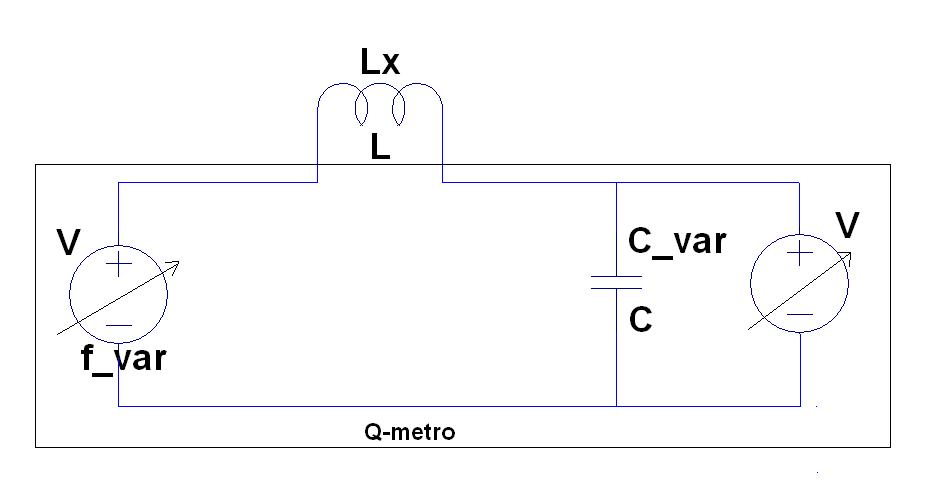
\includegraphics[width=8cm]
				{Imagenes/qmetro.png}
				\caption{Esquema simplificado del Q-metro}
				\label{img001} 
			\end{figure}
		\indent Como es un circuito serie, la máxima corriente se obtiene en 
		la resonancia, dado que la reactancia inductiva de la bobina se 
		cancela con la capacitiva. Si fuesen componentes ideales, la corriente
		sería infinita y los valores de tensiones de la bobina y del capacitor
		serían $+\infty$ y $-\infty$ respectivamente. \\
		\indent Como no son componentes ideales, los mismos tienen pérdidas y
		se las modelizan con una resistencia, por ende, la corriente no es 
		infinita. La respectiva tensión del capacitor en situación de 
		resonancia es $V_c = \frac{X_L\cdot V}{R}$. \\
		\indent Como el valor de Q es $Q=\frac{\omega L}{R}$, se observa que 
		$$V_c = Q \cdot V$$

		\indent La frecuencia de resonancia se la puede determinar de la 
		siguiente forma
		$$|X_L|=|X_C| \Rightarrow w\cdot L = \frac{1}{w\cdot C}$$

		$$f=\frac{1}{2\pi\sqrt{LC}}$$ 
		
		\indent Conocidos los valores de la capacidad, $C$, y la frecuencia, 
		$f$, puede obtenerse el valor de la inductancia de $L_x$ y tambi\'en 
		su resistencia serie equivalente con las siguientes expresiones
		$$L=\frac{1}{(2\pi)^2 f^2C}+\epsilon_L\cdot L$$
		Donde $\epsilon_L=2\epsilon_f+\epsilon_C=2\cdot 1.5\%+\frac{0.1pF}{C}$, 
		puede calcularse a partir de las especificaciones del  fabricante.
		
		$$R_s=\frac{2\pi\cdot f\cdot L}{Q}+\epsilon_{R_s}\cdot R_s$$
		Donde $\epsilon_{R_s}=\epsilon_f+\epsilon_Q= 1.5\%+ 7\%=8.5\%$ se 
		obtiene tambi\'en de las especificaciones del fabricante.
		\\
		\indent En la Tabla \ref{tab:001} se muestran los resultados obtenidos
		para un inductor realizando un barrido de frecuencias.
		
		\begin{table}[!htp]
			\centering
			\begin{tabular}{|c|c|c|c|c|}
				\hline
				Frecuencia & C & Q & L (calculado) & $R_s$ (calculado) \\
				\hline
				$13.3~MHz~\pm1.5\%$& $25~pF~\pm0.1pF$& $182~\pm7\%$ & 
				$5.73~\mu Hy~\pm3.40\%$ &$ 2.63~\Omega~\pm8.5\%$ \\
				\hline
				$10.7~MHz~\pm1.5\%$& $40~pF~\pm0.1pF$& $200~\pm7\%$ & 
				$5.54~\mu Hy~\pm3.25\%$ &$ 1.86~\Omega~\pm8.5\%$ \\
				\hline
				$9.6~MHz~\pm1.5\%$& $50~pF~\pm0.1pF$& $200~\pm7\%$ & 
				$5.50~\mu Hy~\pm3.20\%$ &$ 1.66~\Omega~\pm8.5\%$ \\
				\hline  
				$6.9~MHz~\pm1.5\%$& $100~pF~\pm0.1pF$& $195~\pm7\%$ & 
				$5.33~\mu Hy~\pm3.10\%$ &$ 1.18~\Omega~\pm8.5\%$ \\
				\hline  										
				$4.0~MHz~\pm1.5\%$& $305~pF~\pm0.1pF$& $170~\pm7\%$ & 
				$5.20~\mu Hy~\pm3.03\%$ &$ 0.77~\Omega~\pm8.5\%$ \\
				\hline
				$3.2~MHz~\pm1.5\%$& $470~pF~\pm0.1pF$& $155~\pm7\%$ & 
				$5.17~\mu Hy~\pm3.02\%$ &$ 0.68~\Omega~\pm8.5\%$ \\
				\hline  						  	  
			\end{tabular}
			\caption{Mediciones con el Q-metro} \label{tab:001}
		\end{table}		
		\indent De la Tabla puede observarse que las mediciones de inductancia 
		tienen una incerteza baja (menor al $4\%$ en todos los casos) y que la 
		mayor parte de su incerteza est\'a compuesta por la incerteza de la 
		frecuencia. Con lo cual utilizando un instrumento que determine la 
		frecuencia con menor incerteza (como un frecuenc\'imetro) se mejora 
		notablemente la incertidumbre de la inductancia. Esto se realiza, 
		obteniendose una incerteza menor al $ 1\%$ en todos los casos. \\
		\indent Por otra parte, se observa un incremento de la resistencia
		serie a medidia que se aumenta la frecuencia, con el efecto skin se 
		explica este fenómeno; la sección efectiva del alambre disminuye, 
		logrando así un incremento en la resistencia. Dicha medición se obtiene 
		con una incerteza dominada principlmemente por la incerteza del factor 
		Q (que es el $7\%$). Con lo cual si se desea obtener una incerteza menor
		deber\'a elegirse otro instrumento que no tenga un piso de incertidumbre
		tan grande. \\
		\indent Notar de la Tabla que el valor de Q alcanza un m\'aximo y que 
		luego debe disminuir hasta 0 cuando alcanza la frecuencia de resonancia)
		. \\
	
	\subsection{Mediciones con el RLC}		
		\indent Es importante antes de comenzar a medir con el RLC, realizar su 
		calibraci\'on. De esta forma se consideran y se descuentan las 
		impedancias residuales serie y paralela que se a\~naden a la impedancia 
		a medir debido al cable de conexión. Para ello deben dejarse la puntas 
		del instrumento abiertas (para medir la impedancia paralela residual) y 
		en cortocircuito (para medir la impedancia serie residual). Es 
		importante destacar que dicha corrección lo realiza en todas las 
		frecuencias que se realiza la medición.

		\subsubsection{Inductancia de una bobina con n\'ucleo de aire}
		
		\indent En la Tabla \ref{tabRLCbobina} se puede observar los resultados 
		obtenidos de la medici\'on de una bobina con nucleo de aire a diferentes
		frecuencias, usando el RLC. De ella puede notarse que los valores de 
		inductancia obtenidos son pr\'oximos al de las mediciones realizadas con
		el Q-metro (ver Tabla \ref{tab:001}). Sin embargo, debe notarse que a 
		diferencia de los valores obtenidos con el Q-metro , el RLC tiene una 
		incerteza un orden menor, con lo cual resulta ser un instrumento m\'as 
		exacto. \\
		\indent Pero, por otra parte, posee la desventaja de tener un rango 
		limitado de frecuencias de operaci\'on (desde $12~Hz$ hasta 
		$100.00~kHz$) con lo cual resulta imposible caracterizar su 
		comportamiento en altas frecuencias. \\
		\indent Respecto al valor de la resistencia equivalente, si bien su 
		valor se calcula empleando las f\'ormulas utilizadas previamente, este 
		valor figura en una segunda pantalla del instrumento y su incerteza se 
		especifica al $0.05\%$
		
		\begin{table}[!htp]
			\centering
			\begin{tabular}{|c|c|c|c|}
				\hline
				Frecuencia & Q & L  & R (calculado) \\
				\hline
				$100.000~kHz$& $36.58~\pm0.05\%$ & $5.23~\mu Hy~\pm0.05\%$ &
				$ 89.8~m\Omega$ \\
				\hline
				$66.660~kHz$& $29.44~\pm0.05\%$ & $5.26~\mu Hy~\pm0.05\%$ &
				$ 74.8~m\Omega$ \\
				\hline
				$50.000~kHz$& $25.11~\pm0.05\%$ & $5.29~\mu Hy~\pm0.05\%$ &
				$ 66.2~m\Omega$ \\
				\hline  
				$40.000~kHz$& $22.42~\pm0.05\%$ & $5.31~\mu Hy~\pm0.05\%$ &
				$ 59.5~m\Omega$ \\
				\hline  										
				$28.572~kHz$& $19.07~\pm0.05\%$ & $5.35~\mu Hy~\pm0.05\%$ &
				$ 50.4~m\Omega$ \\
				\hline
				$20.000~kHz$& $16.10~\pm0.05\%$ & $5.40~\mu Hy~\pm0.05\%$ &
				$ 42.1~m\Omega$ \\
				\hline  
				$10.000~kHz$& $10.78~\pm0.05\%$ & $5.46~\mu Hy~\pm0.05\%$ &
				$ 31.8~m\Omega$ \\
				\hline 										
				$1.000~kHz$& $1.36~\pm0.05\%$ & $5.53~\mu Hy~\pm0.05\%$ &
				$ 25.5~m\Omega$ \\
				\hline 	  
			\end{tabular}
			\caption{Mediciones con el RLC} \label{tabRLCbobina}
		\end{table}
				
		\subsubsection{Capacidad de un capacitor electrol\'itico}	
		\indent Para esta medición se realizó un barrido en frecuencia 
		manteniendo la tensión constante y un barrido de tensión manteniendo la
		frecuecia constante. El modelo utilizado en el RLC meter es de un $RC 
		serie$, pero como el modelo real del capacitor es un $RLC serie$, el 
		valor de capacidad obtenido no es el real, por ende es necesario 
		realizar la correción. Para ello, es necesario tomar de a dos muestras
		para determinar los valores $L_s$ y $C_s$, siguiendo la ecuación 
		\ref{eq:001}
		
		\begin{equation}\label{eq:001}
			X_{med} = \frac{1}{\omega_1\cdot c_{med}} = \omega_1\cdot L_s - 
			\frac{1}{\omega_1\cdot C_s}
		\end{equation}
		
		\indent Reescribiendo el sistema de ecuaciones se observa
		
		\[
		\begin{cases} 
			L = \frac{X_1}{\omega_1} + \frac{1}{\omega_1^2\cdot C} \\ 
			\frac{1}{C} = \omega_2^2\cdot L - \omega_2\cdot X_2
		\end{cases}
		\]
		
		\indent Si agregamos la 2º ecuación dentro de la primer ecuación 
		se logra obtener el valor de L

		\begin{align}\label{eq:002}
			L &= \frac{X_1}{\omega_1} + \frac{\omega_2^2}{\omega_1^2}L 
				- \frac{\omega_2}{\omega_1^2}X_2 \nonumber \\ 
			(1 - \frac{\omega_2^2}{\omega_1^2})L &= \frac{X_1}{\omega_1}
				- \frac{\omega_2}{\omega_1^2}X_2 \nonumber \\
			L &= \frac{X_1 - \frac{\omega_2}{\omega_1}X_2}
				{\omega_1(1 - \frac{\omega_2^2}{\omega_1^2})}
		\end{align}

		\indent Utilizando el resultado de la ecuación \ref{eq:002} y la primera
		igualdad de la ecuación \ref{eq:001} resulta

		\begin{equation}\label{eq:003}
			L = \frac{\frac{1}{C_{med1}} - \frac{1}{C_{med2}}}
					{\omega_1^2 - \omega_2^2}
		\end{equation}

		\indent Realizando el mismo procedimiento a partir del sistema de 
		ecuaciones se obtiene el valor de C

		\begin{align}\label{eq:004}
			\frac{1}{C} &= \frac{\omega_1^2}{\omega_2}X_2 + 
				\frac{\omega_1^2}{\omega_2^2}\frac{1}{C} - \omega_1X_1 \nonumber \\
			(1 - \frac{\omega_1^2}{\omega_2^2})\frac{1}{C} &= 
			\frac{\omega_1^2}{\omega_2}X_2 - \omega_1X_1 \nonumber \\
			C &= \frac{1 - \frac{\omega_1^2}{\omega_2^2}}
				{\omega_1(\frac{\omega_1}{\omega_2}X_2 - X_1)}
		\end{align}

		\indent Tomando una vez mas la primer igualdad de la ecuación 
		\ref{eq:001} con el resultado obtenido de \ref{eq:004} se obtiene

		\begin{equation}\label{eq:005}
			C = \frac{\omega_2^2 - \omega_1^2}
				{\frac{\omega_1^2}{C_{med2}} - \frac{\omega_2^2}{C_{med1}}}
		\end{equation}

		\indent Para poder determinar la incertidumbre se utiliza la expresión 
		que se muestra en la ecuación \ref{eq:006}

		\begin{equation}\label{eq:006}
			\Delta f = 	|\frac{\partial f}{\partial x_1}|\Delta x_1 + ... + 
						|\frac{\partial f}{\partial x_n}|\Delta x_n
		\end{equation}

		\indent Las ecuaciones para determinar las incertidumbres absolutas 
		tanto de C como de L se muestran a continuación

		\begin{equation}\label{eq:007}
			\begin{cases}
			\Delta L = (\frac{\Delta C_1}{C_1^2} + \frac{\Delta C_2}{C_2^2}) 
						\frac{1}{\omega_1^2 - \omega_2^2} \\ 
			\Delta C =  \frac{\omega_2^2 - \omega_1^2}{(\frac{\omega_1^2}{C_2} -
						\frac{\omega_2^2}{C_1})^2}(\Delta C_1\frac{\omega_2^2}
						{C_1^2} + \Delta C_2 \frac{\omega_1^2}{C_2^2})
			\end{cases}
		\end{equation}

		\indent En la tabla \ref{tab:002} se muestran los valores obtenidos 
		realizando un barrido en frecuencia con la tensión fija sin 
		polarización, y en la tabla \ref{tab:003} realizándolo en tensión 
		dejando la frecuencia fija a 100Hz. \\
		\indent Respecto a las incertidumbres de las mediciones, la pantalla las
		especifica al 0.05\%. 

		\begin{table}[!htp]
			\centering
			\begin{tabular}{|c|c|c|c|c|}
				\hline
				Frecuencia [KHz] & $C_{med}~\mu F$ & $\Delta C~\mu F$ & 
				$R_{med}~\Omega$ & $\Delta R~\Omega$ \\
				\hline
				0.012 &	207.1 & 0.1 & 1.9 & 0.1 \\
				\hline
				0.120 &	198.7 & 0.1 & 0.57 & 0.01 \\
				\hline
				0.500 &	190.1 & 0.1 & 0.38 & 0.01 \\
				\hline
				1.000 &	186.1 & 0.1 & 0.35 & 0.01 \\
				\hline
				10.00 &	153.82 & 0.08 & 0.30 & 0.01 \\
				\hline
				20.00 &	126.36 & 0.07 & 0.30 & 0.01 \\   
				\hline
				40.00 &	78.31 & 0.04 & 0.30 & 0.01 \\
				\hline
				50.00 &	61.13 & 0.04 & 0.30 & 0.01 \\
				\hline
				66.66 &	41.44 & 0.03 & 0.29 & 0.01 \\
				\hline
				100.0 &	21.71 & 0.02 & 0.29 & 0.01 \\
				\hline	  
			\end{tabular}
			\caption{Barrido en frecuencia del capacitor electrolítico con RLC 
			meter.} 
			\label{tab:002}
		\end{table}	
		
		\begin{table}[!htp]
			\centering
			\begin{tabular}{|c|c|c|c|c|}
				\hline
				Tensión [V] & $C_{med}~[\mu F]$ & $\Delta C~[\mu F]$ & 
				$R_{med}~[K\Omega]$ & $\Delta R~[\Omega]$\\
				\hline
				25 &	209 & 0.1 & 0.660 & 0.4 \\
				\hline
				22.3 &	206 & 0.1 & 0.651 & 0.4 \\
				\hline
				13.8 &	202 & 0.1 & 0.634 & 0.4 \\
				\hline
				6.9 &	201 & 0.1 & 0.632 & 0.4 \\
				\hline
				2.6 &	199 & 0.1 & 0.628 & 0.4 \\
				\hline
				0.6 &	199 & 0.1 & 0.625 & 0.4 \\
				\hline	  
			\end{tabular}
			\caption{Barrido de tensión del capacitor electrolítico con RLC 
			meter.} 
			\label{tab:003}
		\end{table}	

		\indent Utilizando valores contínuos de capacidades medidas de la tabla
		\ref{tab:002} y \ref{tab:003} en las ecuaciones mencionadas anteriormente
		(\ref{eq:003}, \ref{eq:005} y \ref{eq:007}) se obtienen los valores de
		la capacidad e inductancia serie del modelo RLC serie del capacitor. \\
		\indent La tabla \ref{tab:004} muestra cómo varían dichos parámetros en 
		función de la frecuencia y la tabla \ref{tab:003} en función de la 
		tensión.
		
		\begin{table}[!htp]
			\centering
			\begin{tabular}{|c|c|c|c|c|c|c|}
				\hline
				Frecuencia [KHz] & $C_s~[\mu F]$ & $\Delta C_s~[\mu F]$ & 
				$L_s~[\mu Hy]$  & $\Delta L_s~[\mu Hy]$  & $R_s~[\Omega]$ & 
				$\Delta R_s~[\Omega]$ \\
				\hline
				0.012 - 0.120 &	207.1 & 0.1 & -358 & 9 & 1.24 & 0.07 \\
				\hline
				0.120 - 0.500 &	199.3 & 0.2 & -24.5 & 0.6 & 0.48 & 0.03 \\
				\hline
				0.500 - 1.000 &	191.5 & 0.2 & -3.9 & 0.2 & 0.37 & 0.02 \\
				\hline
				1.000 - 10.00 &	186.5 & 0.1 & -0.289 & 0.002 & 0.33 & 0.02 \\
				\hline
				10.00 - 20.00 &	165.8 & 0.2 & -0.1195 & 0.0007 & 0.30 & 0.02 \\
				\hline
				20.00 - 40.00 &	158.7 & 0.2 & -0.1025 & 0.0003 & 0.30 & 0.02 \\
				\hline
				40.00 - 50.00 &	157 & 1 & -0.1012 & 0.0005 & 0.30 & 0.02 \\
				\hline
				50.00 - 66.66 &	158 & 2 & -0.1015 & 0.0004 & 0.30 & 0.02 \\
				\hline
				66.66 - 100.0 &	151 & 2 & -0.1000 & 0.0003 & 0.29 & 0.02 \\
				\hline	  
			\end{tabular}
			\caption{Parámetros del capacitor en función de la frecuencia.} 
			\label{tab:004}
		\end{table}	
		
		\indent Como se puede apreciar en la tabla \ref{tab:004}, $L_s$ dió 
		negativa, esto no tiene sentido físico. Se cometió un error grosero en 
		la medición, la cual fue no calibrar el RLC para que anule los efectos 
		del cable de conexión. Por lo tanto el modelo del circuito a medir ya no
		es más el equivalente de solo un capacitor. \\
		\indent En la tabla \ref{tab:003} se midió cómo varía la capacidad en 
		función de la tensión, como se hizo a una frecuencia de 100 Hz, se puede
		despreciar el efecto inductivo que tiene el modelo, dado que es a una 
		frecuencia menor a la resonancia serie. Se puede apreciar una variación 
		bastante apreciable, alrededor del 5\% del valor total.
		
		\subsubsection{Capacidad de un capacitor cer\'amico}
		\indent Las mediciones son realizadas utilizando el mismo procedimiento
		que en la sección anterior, barrido en frecuencia dejando la tensión 
		fija y barrido en tensión dejando la frecuencia fija en 100 KHz esta 
		vez. \\
		
		\indent Las fórmulas para calcular la $L_s$, $C_s$ y sus incertidumbres 
		son las ecuaciones \ref{eq:003}, \ref{eq:005} y \ref{eq:007} 
		respectivamente. \\
		\indent Las tablas \ref{tab:006} y \ref{tab:007} muestran los resultados
		de las mediciones 
	
		\begin{table}[!htp]
			\centering
			\begin{tabular}{|c|c|c|c|c|}
				\hline
				Frecuencia [KHz] & $C_{med}~[nF]$ & $\Delta C~[nF]$ & 
				$R_{med}~[\Omega]$ & $\Delta R~[\Omega]$ \\
				\hline
				0.012 &	23.88 & 0.02 & 23.33 & 0.01 \\
				\hline
				0.120 &	23.29 & 0.02 & 0.76 & 0.01 \\
				\hline
				0.500 &	23.18 & 0.02 & 0.134 & 0.01 \\
				\hline
				1.000 &	23.10 & 0.02 & 0.064 & 0.001 \\
				\hline
				10.00 &	22.82 & 0.02 & 0.007 & 0.001 \\
				\hline
				20.00 &	22.71 & 0.02 & 0.0035 & 0.001 \\
				\hline
				40.00 &	22.54 & 0.02 & 0.0018 & 0.001 \\
				\hline
				50.00 &	22.48 & 0.02 & 0.0015 & 0.001 \\
				\hline
				66.666 & 22.44 & 0.02 & 0.0012 & 0.001 \\
				\hline
				100.0 &	22.53 & 0.02 & 0.001038 & 0.000001 \\
				\hline
			\end{tabular}
			\caption{Barrido de frecuencia del capacitor cerámico con RLC 
			meter.} 
			\label{tab:006}
		\end{table}	

		\begin{table}[!htp]
			\centering
			\begin{tabular}{|c|c|c|c|c|}
				\hline
				Tensión [V] & $C_{med}~[nF]$ & $\Delta C~[nF]$ & 
				$R_{med}~[K\Omega]$ & $\Delta R~[K\Omega]$\\
				\hline
				25 &	19.01 & 0.02 & 1.26 & 0.01 \\
				\hline
				22.3 &	19.51 & 0.02 & 1.24 & 0.01 \\
				\hline
				13.8 &	22.02 & 0.02 & 1.29 & 0.01 \\
				\hline
				6.9 &	22.22 & 0.02 & 1.27 & 0.01 \\
				\hline
				2.6 &	23.20 & 0.02 & 1.3 & 0.01 \\
				\hline
				0.6 &	23.25 & 0.02 & 1.23 & 0.01 \\
				\hline	  
			\end{tabular}
			\caption{Barrido de tensión del capacitor cerámico con RLC 
			meter.} 
			\label{tab:007}
		\end{table}	
		
		\indent Utilizando valores contínuos de capacidades medidas de la tabla
		\ref{tab:006} y \ref{tab:007} en las ecuaciones mencionadas anteriormente
		(\ref{eq:003}, \ref{eq:005} y \ref{eq:007}) se obtienen los valores de
		la capacidad e inductancia serie del modelo RLC serie del capacitor. \\
		\indent La tabla \ref{tab:008} muestra cómo varían dichos parámetros en 
		función de la frecuencia.
		
		\begin{table}[!htp]
			\centering
			\begin{tabular}{|c|c|c|c|c|c|c|}
				\hline
				Frecuencia [KHz] & $C_s~\mu F$ & $\Delta C_s~[pF]$ & 
				$L_s~mHy$  & $\Delta L_s~mHy$  & $R_s~\Omega$ & 
				$\Delta R_s~\Omega$ \\
				\hline
				0.012 - 0.120 &	23.89 & 21 & -1885 & 128 & 1.9 & \\
				\hline
				0.120 - 0.500 &	23.30 & 23 & -22 & 8 & 0.57 & \\
				\hline
				0.500 - 1.000 &	23.21 & 34 & -5 & 3 & 0.38 & \\
				\hline
				1.000 - 10.00 &	23.10 & 21 & -0.14 & 0.02 & 0.35 & \\
				\hline
				10.00 - 20.00 &	22.86 & 34 & -0.0179 & 0.007 & 0.3 & \\
				\hline
				20.00 - 40.00 &	22.77 & 34 & -0.007 & 0.002 & 0.3 & \\   
				\hline
				40.00 - 50.00 &	22.65 & 93 & -0.003 & 0.003 & 0.3 & \\
				\hline
				50.00 - 66.66 &	22.53 & 72 & -0.001 & 0.001 & 0.3 & \\
				\hline
				66.66 - 100.0 &	22.37 & 52 & 0.0008 & 0.0003 & 0.29 & \\
				\hline	  
			\end{tabular}
			\caption{Parámetros del capacitor en función de la frecuencia.} 
			\label{tab:008}
		\end{table}	

		\indent Como se puede apreciar, también la inductancia calculada 
		presenta un valor negativo, se le atribuye al mismo error grosero 
		cometido anteriormente, dado que ambas mediciones se realizaron de forma
		continuada. \\ 
		\indent En la medición de la respuesta en función de la variación de 
		tensión de alimentación no se observan cambios apreciables en los 
		parámetros, a diferencia del capacitor electrolítico, en el cual la 
		variación era del 5\%.
	
	\subsection{Mediciones con el puente de impedancias}
		\subsubsection{Inductancia de una bobina con n\'ucleo de aire}
		\indent Para esta medición se conectó directamente la bobina al puente, 
		dicho instrumento acepta que se le pueda conectar un generadore externo.
		\\
		\indent El procedimiento de medición es el siguiente, una vez conectada
		la impedancia al puente, se modifican 2 resistencias, una equilibrando
		la parte activa y la otra la reactiva del puente, con el objetivo de 
		balancear dicho circuito. \\
		\indent Dicho procedimiento debe ser iterativo, primero se intenta 
		balancear la parte activa, luego la reactiva; se repiten dichos pasos
		hasta lograr que el puente quede definitivamente balanceado. En la 
		tabla \ref{tabPUENTEbobina} se muestran las mediciones obtenidas. \\
		\indent Con respecto a las incertidumbres de las respectivas mediciones,
		la incertidumbre absoluta de la lectura de L es 
		$$\Delta L = \pm (0.1\%~rdg +0.01\%~fs +0.2\%rdg~on~lowest~range)$$
		\indent La incertidumbre de la medición de Q es 
		$$\Delta Q = \pm5\%~rdg$$

		\begin{table}[!htp]
			\centering
			\begin{tabular}{|c|c|c|c|c|c|c|}
				\hline
				Frecuencia & Q & $\Delta Q$ & L & $Delta L$  & $R_s$ & 
				$\Delta R_s $ \\
				\hline
				$20~kHz$& 20 & 1 & $5.10~\mu Hy$ & $0.02~\mu Hy$ & 
				$ 32~m\Omega$ & $2~m\Omega$\\
				\hline
				$1~kHz$& 1.8 & 0.09 & $6.30~\mu Hy$ & $0.02~\mu Hy$ & 
				$ 22~m\Omega$ & $2~m\Omega$\\
				\hline	  
			\end{tabular}
			\caption{Mediciones con el puente de impedancias.} 
			\label{tabPUENTEbobina}
		\end{table}	
		
		\indent Para poder calcular la resistencia serie se procedió a utilizar 
		la fórmula del Q, la cual es 

		$$Q = \frac{X_L}{R_s}$$

		\indent La incertidumbre de dicha medición es sencillamente la suma de 
		las incertidumbres relativas de las mediciones. \\
		\indent Se puede apreciar que el valor de la inductancia varía con 
		respecto a la frecuencia. \\
		\indent Cabe destacar que el valor $R_s$ posee alrededor del 10\% de 
		incertidumbre, el cual es un valor bastante considerable. \\
		\indent En el caso particular de esta bobina con núcleo de aire, se 
		debería desechar cualquier medición de L, dada la incertidumbre de la 
		medición y que el la frecuencia máxima del RLC meter es solo de 100 KHz,
		en cambio, la frecuencia de autorresonancia medida con el Q metro en el 
		siguiente apartado resulta de 35.44MHz, por ende, 100KHz es una 
		frecuencia muy chica con respecto a la frecuencia a la que se trabaja 
		con dicha bobina.

	\subsection{Mediciones con el impedanc\'imetro}
		
		\indent Hay igual que con el RLC es necesario calibrar el 
		impedanc\'metro antes de realizar una medici\'on usando socket Probe 
		Check. \\
		\indent Con este instrumento, para mediciones de resistencia la 
		incerteza absoluta se calcula como
		\begin{equation}\label{modulo}
			\Delta R=\pm 4\%\cdot R_{fe}\pm(\frac{f}{30~MHz}+\frac{R}{25~k
			\Omega})\%\cdot R_{med}
		\end{equation}
		
		\indent Mientras que para mediciones de \'angulo la incerteza absoluta 
		se calcula como
		
		\begin{equation}\label{angulo} 
			\Delta\phi=\pm(3+\frac{f}{30~MHz}+\frac{R}{25~k\Omega})
		\end{equation}
		
		\indent Por otra parte las mediciones de impedancia incluyen tambi\'en 
		efectos resuidales a la impedancia $Z_x$ que se desea medir. Este error 
		sistem\'atico se puede observar en la Figura \ref{impres}, notando que 
		incluye una impedancia serie $Z_s=0.5\Omega+j\cdot\omega\cdot8nHy$ y una
		admitancia en paralelo a $Z_x$ de $Y_p=j\cdot\omega\cdot0.3pF$
		
		\begin{figure}[!htb]
			\centering
			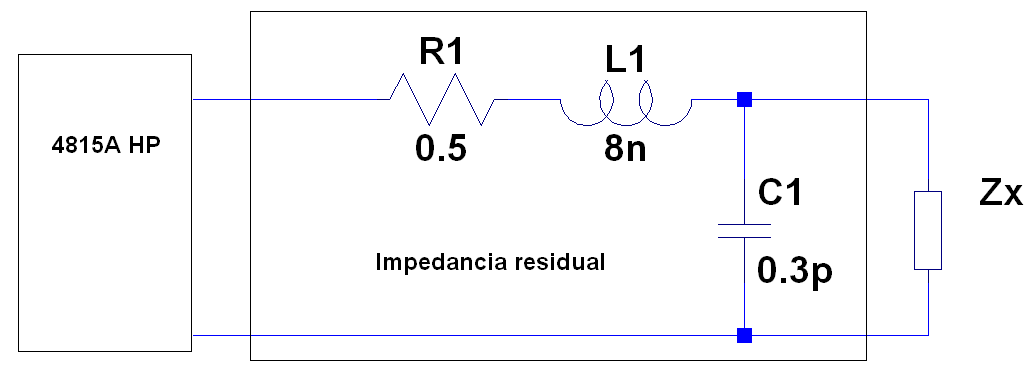
\includegraphics[width=8cm]
			{Imagenes/impedanciares.png}
			\caption{Impedancia residual del impedanc\'imetro.}
			\label{impres} 
		\end{figure}
		
		\indent De esta forma es posible eliminar este error sistem\'atico y 
		obtener el valor de $Z_x$, a partir del valor medido, $Z_m$, mediante la
		siguiente expresi\'on
		
		$$Z_x=\frac{Z_m-Z_s}{1-Y_p(Z_m-Z_s)}$$
		
		\subsubsection{Frecuencia de resonancia de una bobina con n\'ucleo de 
		aire}
		
		\indent La frecuencia de resonancia se obtiene cuando la parte reactiva 
		de la impedancia a medir tiene fase nula, es decir, cuando
		
		$$\omega\cdot L=\frac{1}{\omega \cdot C}$$
		
		\indent Con lo cual, conocida la frecuencia de resonancia y asumiendo 
		que la inductancia no var\'ia demasiado con la frecuencia puede 
		obtenerse la capacidad equivalente del modelo (el cual se puede observar
		en la Figura \ref{inductorequiv}). De esta manera
		
		$$C=\frac{1}{\omega^2 \cdot L}+\epsilon_C \cdot C$$
		%\todo[inline]{no se de donde sacaste la L medida o calculada, si me pongo a 
	%	corregir esto agregaría la tabla de las mediciones de la %impedancia con
		%el ángulo medido con el impedancimetro, es eso o que quede asi, no se, 
	%	ya estoy podrido de este puto informe..}
		\indent Donde $\epsilon_C=2\epsilon_w+\epsilon_L\approx \epsilon_L =
		3.40\%$, ya que la incerteza de la frecuencia (obtenida con un 
		frecunec\'imetro) es mucho menor a la de la inductancia (obtenida con el
		Q-metro en $f=13.3~MHz$, como se muestra en la Secci\'on \ref{inductancia}) \\
		\indent De esta manera se hall\'o la frecuencia ($f_{resonancia}=
		35.440~MHz$) para la cual es obtuvo fase nula y se calcul\'o la 
		capacidad equivalente
		
		$$C=\frac{1}{(2\pi 35.440~MHz)^2 \cdot L}\pm \epsilon_C \cdot C=3.52pF \pm~3.40\%$$
		\begin{figure}[!htb]
			\centering
			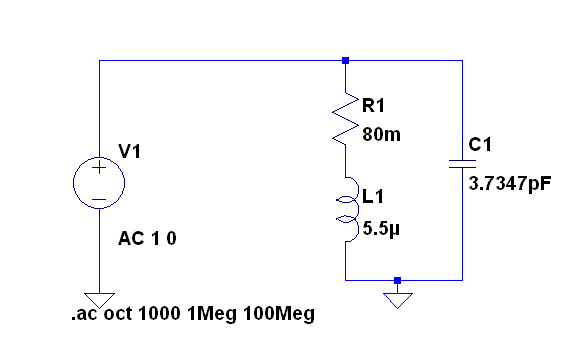
\includegraphics[width=8cm]
			{Imagenes/induceqquiv.png}
			\caption{Modelo equivalente del inductor.}
			\label{inductorequiv} 
		\end{figure}
		
		\indent En la Figura \ref{respfreq} se puede observar una simulaci\'on 
		realizada con el modelo equivalente, donde se puede observar la 
		impedancia en funci\'on de la frecuencia y la resonancia en 
		$f_{resonancia}$.
		
		\begin{figure}[!htb]
			\centering
			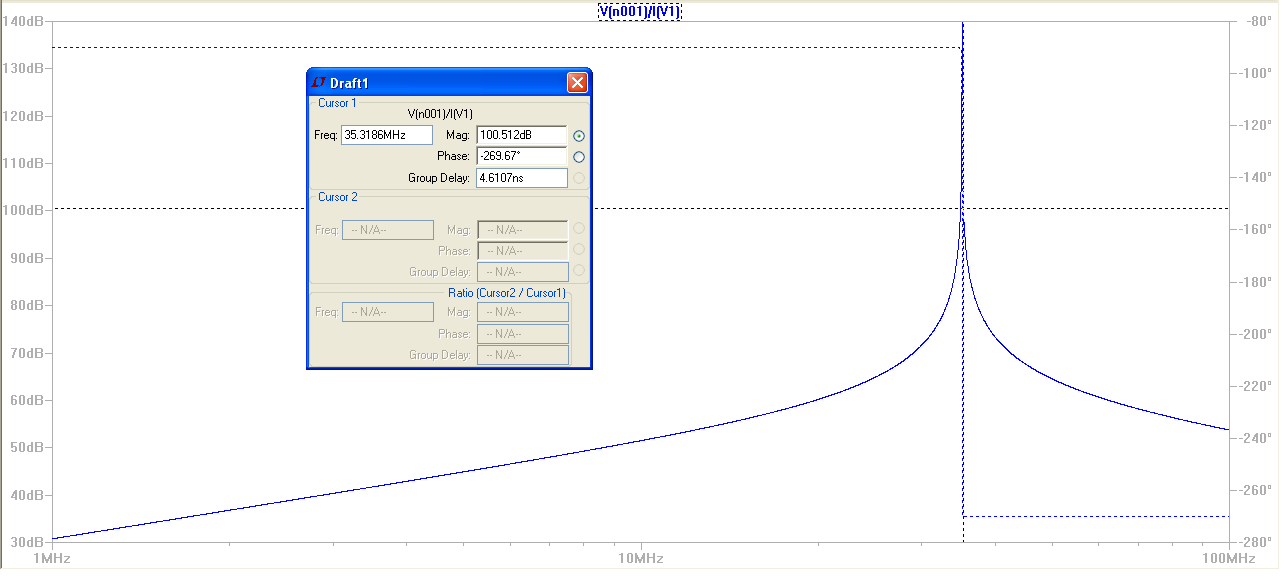
\includegraphics[width=9cm]
			{Imagenes/respfreq.png}
			\caption{Respuesta en frecuencia t\'ipica de un inductor.}
			\label{respfreq} 
		\end{figure}
		
		\subsubsection{Inductancia de una bobina con n\'ucleo de ferrite}
		
		\indent En la Tabla \ref{tabIMPbobina} se muestran los resultados 
		obtenidos en m\'odulo y fase para un barrido en frecuencia entre 
		$25~MHz$ a $100~MHz$. Debe notarse que hasta una frecuencia de  $42~MHz$
		, la bobina contin\'ua comport\'andose como un inductor de inductancia 
		$L=\frac{\left|Z\right|}{2\pi\cdot f}~\pm~\epsilon_L\cdot L$. Donde 
		$\epsilon_L=\epsilon_f+\epsilon_{\left|Z\right|}\approx
		\epsilon_{\left|Z\right|}$
		
		\begin{table}[!htp]
			\centering
			\begin{tabular}{|c|c|c|c|}
				\hline
				Frecuencia & $\left|Z\right|~[\Omega]$ & $arg(Z)~[º]$ & 
				$L (calculado)~[\mu Hy]$\\
				\hline
				$25.5~MHz$ & $160\pm14$ & $90\pm4$ & $0.99\pm0.2$ \\
				\hline
				$42~MHz$ & $260\pm16$ & $90\pm5$ & $0.98\pm0.2$\\
				\hline
				$44.8~MHz$ & $300\pm45$ & $85\pm5$ & $1.06\pm0.3$ \\
				\hline
				$58.2~MHz$ & $430\pm49$ & $78\pm5$ & $1.17\pm0.3$ \\
				\hline									
				$69.5~MHz$ & $560\pm53$ & $72\pm6$ & $1.28\pm0.3$ \\
				\hline									
				$80.0~MHz$& $640\pm58$ & $55\pm6$ & $1.27\pm0.3$ \\
				\hline									
				$84.0~MHz$ & $550\pm56$ & $45\pm6$ & $1.04\pm0.3$ \\
				\hline									
				$93.0~MHz$ & $430\pm54$ & $70\pm7$ & $0.73\pm0.2$ \\
				\hline									
				$100.0~MHz$ & $750\pm66$ & $65\pm7$ & $1.19\pm0.3$ \\
				\hline			
			\end{tabular}
			\caption{Mediciones con el impedanc\'imetro de una bobina con 
			n\'ucleo de ferrite} \label{tabIMPbobina}
		\end{table}	
		
		\indent Si se utiliza la f\'ormula para eliminar el error sistem\'atico 
		de la medic\'on se obtiene que (para la frecuencia de 42 MHz, donde 
		todav\'ia se comporta como un inductor)
		
		$$Z_x=-0.48\Omega+j\cdot 252\Omega$$
		
		\indent Es decir, se obtiene una inductancia de $L=0,96 \mu F$ y una 
		resistencia negativa, la cual probablemente se deba a la incerteza del 
		instrumento en la fase ocacionando que el fasor de impedancia que 
		idealmente tiene una fase de 90 grados, tenga una parte real negativa. 
		Se puede concluir que no es un buen instrumento para medir la 
		resistencia serie equivalente de un inductor, pero si lo es para medir 
		inductancias. \\
		\indent Por otra parte debe notarse que el barrido en frecuencia 
		continua luego de los 42 MHz, sin embargo no se llega a alcanzar la 
		frecuencia de resonancia donde la fase es nula. Es decir que la 
		transici\'on de fase no es abrupta, lo cual indica que la resistencia 
		serie es de mayor orden que la de la bobina con n\'ucleo de aire. 

		\subsubsection{Param\'etros de una l\'inea de transmisi\'on}
		
		\indent Como la impedancia de entrada de una l\'inea de transmisi\'on 
		(la que mide el impedanc\'imetro) est\'a dada por 
		
		$$Z_{in}=Z_0\frac{Z_L+Z_0\tanh(\gamma L)}{Z_0+Z_L\tanh(\gamma L)}$$
		
		\indent Suponiendo que la l\'inea es de bajas p\'erdidas 
		$\gamma=\alpha+j\beta=j\beta=j\frac{2\pi}{\lambda}$ y si adem\'as se 
		impone la condici\'on de que $L=\frac{\lambda}{8}$ entonces la 
		expresi\'on de la impedancia de entrada se reduce a la siguiente
		
		$$Z_{in}=Z_0\frac{Z_L+jZ_0}{Z_0+jZ_L}$$
		
		\indent Si $Z_L= 0$ entonces $Z_{in}=jZ_0$ \\
		\indent Si $Z_L \rightarrow \infty$ entonces $Z_{in}\rightarrow-jZ_0$.\\
		\indent Entonces conectando una l\'inea al impedanc\'imetro a una 
		frecuencia adecuada y dejando el extremo libre de la l\'inea 
		cortocircuitado o abierto se obtiene el valor de la impedancia de la 
		l\'inea, la cual es de 
		$Z_0=75~\Omega~\pm~4.3\Omega$ ($f=7.9~MHz$ $L=3~m~\pm~0.05m$) \\
		
		\indent Por otra parte se si se elije 
		$L=\frac{\lambda}{2},3\frac{\lambda}{2}, 5\frac{\lambda}{2} ...$ y que 
		$Z_L\rightarrow\infty$, entonces puede obtenerse la atenuaci\'on de la 
		l\'inea
		
		$$Z_{in}=Z_0\frac{Z_L+Z_0\alpha L}{Z_0+Z_L\alpha L}=\frac{Z_0}{\alpha L}$$
		
		\indent Despejando la atenuaci\'on de la l\'inea se obtiene (y agregando
		las incertezas)
		
		$$\alpha=\frac{Z_0}{Z_{in} L}~\pm~\epsilon_{\alpha}\cdot\alpha$$
		
		\indent Con $\epsilon_{\alpha}=\epsilon_{Z_0}+\epsilon_{Z_{in}}+
		\epsilon_{L}$ o la atenuaci\'on en decibles cada $100~m$
		
		$$\alpha=\frac{100~m\cdot Z_0\cdot8.69~dB}{Z_{in}\cdot L}~\pm~
		\epsilon_{\alpha}\cdot \alpha$$
		
		\indent Con la misma l\'inea con la que se obtuvo $Z_0$ y a una 
		frecuencia de $32~MHz$ se obtuvo una $Z_{in}=(2750\pm153)~\Omega$ con
		lo cual $\alpha = (7.90\pm1.02)\frac{dB}{100m} $ \\
		\indent A una frecuencia mayor, de $100~MHz$ se obtuvo una 
		$Z_{in}=(1350~\pm166)\Omega$ con lo cual 
		$\alpha = (16.09\pm3.16)\frac{dB}{100m}$\\
		\indent Como se puede observar al aumentar la frecuencia de operaci\'on 
		la atenuac\'on en la l\'inea no es constante sino que aumenta.
		
		\subsubsection{Par\'ametros de un cristal}	
		
		\indent Un cristal se lo puede modelar como un capacitor en paralelo a 
		múltiples circuitos RLC serie, cada uno representa un modo de resonancia
		distinto, a efectos de este trabajo práctico sólo se lo modelará con un 
		único modo de resonancia, como se muestra en la figura \ref{img004}

		\begin{figure}[!htb]
			\centering
			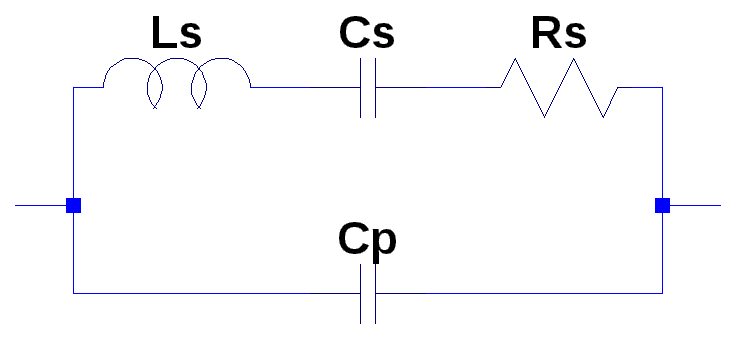
\includegraphics[width=8cm]{Imagenes/esqXtal.png}
			\caption{Esqemático simplificado del cristal.}
			\label{img004} 
		\end{figure}

		\indent Dicho circuito equivalente posee dos frecuencias de resonancia,
		una serie y otra paralelo, ambas muy cercanas entre sí. La resonancia 
		serie es la menor de las dos, en dicho punto la fase de la impeancia es
		igual a 0, por ende, puede medirse directamente la resistencia serie 
		$R_s$. \\
		\indent Como generalmente la resistencia de la resonancia serie es muy 
		chica, hay que restar $0.5\Omega$ del efecto de carga de la punta. \\
		\indent Un gráfico típico de la impedancia de entrada de un cristal en 
		función de la frecuencia se observa en la imagen \ref{img005}.
		
		\begin{figure}[!htb]
			\centering
			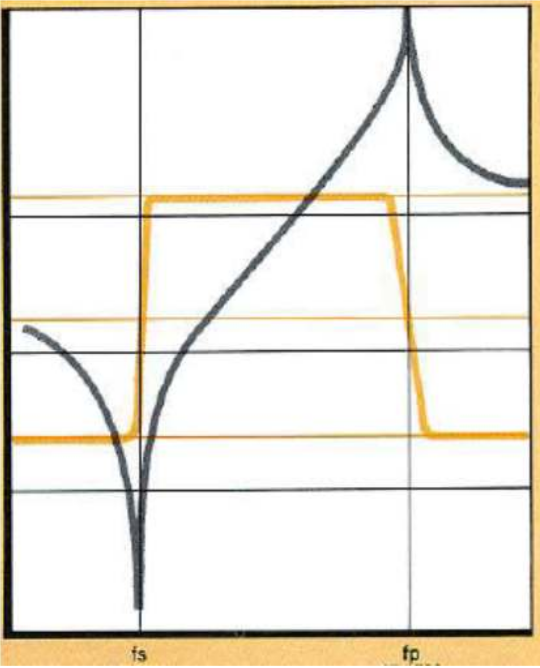
\includegraphics[width=8cm]{Imagenes/curvaCaractXtal.png}
			\caption{Curva característica del xtal.}
			\label{img005} 
		\end{figure}

		\indent Se puede observar que el circuito se comporta como un capacitor
		a frecuencias menores que la de la resonancia serie, dicho capacitor es 
		aproximadamente igual a $C_p$ dado que $C_s$ es mucho menor. \\
		\indent Las otras fórmulas utilizadas para realizar los cálculos del 
		resto de los parámetros del xtal son las siguientes.
	
		\begin{equation} \label{eq001}
			C_p = \frac{1}{2\omega\cdot x_c}		
		\end{equation}
		
		\begin{equation} \label{eq002}
			C_s = C_p \frac{2\cdot(f_p - f_s)}{f_p}
		\end{equation}

		\begin{equation} \label{eq003}
			L = \frac{1}{4\pi^2f_s^2C_s}
		\end{equation}

		\indent Donde $f_s$ y $f_p$ son las frecuencias de resonancia serie y 
		paralelo respectivamente. \\
		\indent A la hora de medir el Q del cristal se determina utilizando el 
		método del ancho de banda, el cual consiste en medir las frecuencias 
		donde la potencia de salida disminuye unos $3~dB$, o que es lo mismo, 
		si se trata de un polo simple como este caso, hay un defasaje de $45º$.
		Por lo tanto Q queda determinado de la siguiente forma
		
		\begin{equation} \label{eq004}
			Q = \frac{f_0}{\Delta f_{\pm45}}
		\end{equation}
		
		\indent Para realizar la medición de los parámetros se utiliza el 
		impedancímetro vectorial (HP 4815A), el cual mide la fase y el módulo de
		la impedancia. Los valores obtenidos se vuelcan en la tabla \ref{tab003}
		
		\begin{table}[!htp]
			\centering
			\begin{tabular}{|c|c|c|c|c|}
				\hline
				Frecuencia [MHz] & |Z| & $\Delta |Z|$ & arg(Z) [º] & 
				$\Delta arg(Z)~[º]$ \\
				\hline
				18.9960000 & $2.85~K\Omega$ & 150 & $-90^{\circ}$ & 4 \\
				\hline
				19.9948400 & - & - & $-45^{\circ}$ & 4 \\ 
				\hline
				19.9950580 & $17~\Omega$ & 2 & $0^{\circ}$ & 4 \\
				\hline
				19.9952860 & - & - & $45^{\circ}$ & 4 \\ 
				\hline									
				20.0311383 & $560~\Omega$ & 44 & $45^{\circ}$ & 4 \\
				\hline									
				20.0311556 & $640~\Omega$ & 45 & $0^{\circ}$ & 4 \\
				\hline									
				20.0311634 & $550~\Omega$ & 44 & $-45^{\circ}$ & 4 \\
				\hline									
			\end{tabular}
			\caption{Mediciones con el impedancímetro vectorial} \label{tab003}
		\end{table}	
		
		\indent Utilizando los datos medidos obtenidos en la tabla \ref{tab003}
		y las ecuaciones \ref{eq001}, \ref{eq002}, \ref{eq003} y \ref{eq004} se
		obtienen los parámetros del cristal, mostrados en la tabla \ref{tab004}
		
		\begin{table}[!htp]
			\centering
			\begin{tabular}{|c|c|c|}
				\hline
				Parámetro & Valor & Incertidumbre absoluta \\
				\hline
				$C_p$ & $2.9~pF$ & 0.2 \\
				\hline
				$C_s$ & $10.6~fF$ & 0.6 \\ 
				\hline
				$L_s$ & $6.0~mHy$ & 0.3 \\
				\hline
				$R_s$ & $16.5~\Omega$ & 1.3 \\ 
				\hline									
				$Q_p$ & $798054$ & - \\
				\hline
				$Q_s$ & $44832$  & - \\
				\hline
			\end{tabular}
			\caption{Mediciones con el impedancímetro vectorial} \label{tab004}
		\end{table}	

		\indent Si bien se utilizó un generador externo para la medición del Q 
		del xtal, dado que posee una estabilidad mucho mayor al generador 
		interno del impedancímetro, resultó muy dificultoso realizar las 
		mediciones donde la fase está en la posicion de $\pm45º$. Esto se debe 
		en gran parte que el Q es muy alto, por ende en un $\Delta f$ muy chico 
		cambia mucho la fase. Se puede observar que en la resonancia paralelo el
		cristal posee un Q mucho más alto, por ende la estabilidad del mismo es 
		mucho mayor con respecto a la serie.

		\subsubsection{Mediciones en un circuito activo}
		
		\indent Para realizar la medición de un circuito activo utilizando el 
		impedancímetro vectorial hay que tener varias consideraciones en cuenta.
		
		\begin{itemize}
			\item El nivel de señal del punto de medición debe estar en la zona 
			lineal de funcionamiento del circuito, dado que la impedancia sólo 
			se define para circuitos lineales.
			\indent Todas las mediciones con el impedancímetro vectorial 4815A 
			deben ser referenciadas a tierra.
		\end{itemize}
		
		\indent El circuito a medir es el mostrado en la figura \ref{img006} y 
		particularmente el punto de medición es la entrada del mismo. \\
		\indent Con respecto a la respuesta del mismo, entre las frecuencias 
		de 4 a 6 MHz presenta una resistencia negativa, particularmente en el 3º
		cuadrante del plano de impedancias. Como el impedancímetro mide fase y
		módulo, puede realizar dicha medición sin problemas.
		
		\begin{figure}[!htb]
			\centering
			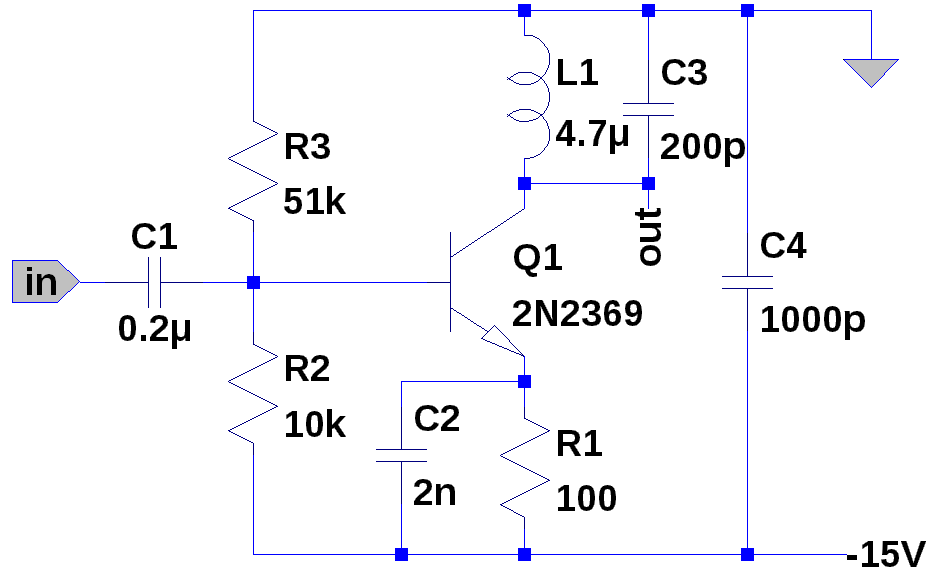
\includegraphics[width=8cm]{Imagenes/ActiveCircuit.png}
			\caption{Circuito activo a medir.}
			\label{img006} 
		\end{figure}

		\indent Se fue haciendo un barrido en frecuencia en el rango indicado,
		y se midió la fase y la impedancia del circuito en dicho punto. La 
		tabla \ref{tabbla} muestra los resultados

		\begin{table}[!htp]
			\centering
			\begin{tabular}{|c|c|c|c|c|}
				\hline
				Frecuencia [kHz] & $X_{med}~[K\Omega]$ & 
				$\Delta X_{med}~[K\Omega]$ & angulo [º] & $\Delta angulo~[º]$ \\
				\hline
				4500.04 & 5.2 & 0.4 & -78 & 4 \\
				\hline
				4800.04 & 5.4 & 0.4 & -95 & 4 \\ 
				\hline
				5200.04 & 2.6 & 0.2 & -162 & 4 \\
				\hline
				5500.05 & 1.05 & 0.2 & -122 & 4 \\ 
				\hline									
				5800.04 & 1.2 & 0.2 & -98 & 4 \\
				\hline
				6000.01 & 1.25 & 0.2 & -96 & 4 \\
				\hline
			\end{tabular}
			\caption{Mediciones de la entrada del circuito con el 
			impedancímetro vectorial} \label{tabbla}
		\end{table}
		
		\subsubsection{Medición de un capacitor cerámico}
		\indent A continuación se realizó la medición de un capacitor cerámico
		de 22 nF, para ello, se colocó directamente el capacitor en la punta 
		del impedancímetro. Como el equivalente del mismo es un circuito RLC 
		serie, como se muestra en la Figura \ref{imagenCapacitor} 
		
		\begin{figure}[!htb]
			\centering
			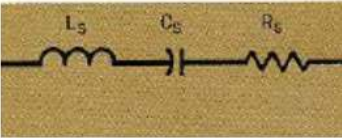
\includegraphics[width=8cm]{Imagenes/EsqCapacitor.png}
			\caption{Modelo Equivalente del capacitor.}
			\label{imagenCapacitor} 
		\end{figure}
		
		Se debe buscar la frecuencia de resonancia, en este punto se anulan la 
		parte activa de la impedancia, por ende la impedancia resultante posee
		fase 0. Se midió cuando hay $\pm 45º$ y en una frecuencia donde las fases
		son $\pm 90º$ para determinar la inductancia y capacidad del equivalente.
		\\
		\indent La tabla \ref{unaTab} muestra los valores medidos con sus 
		respectivas incertidumbres. \\
		\indent Para determinar la incertidumbre de la medición se utiliza la 
		fórmula del manual mostradas en las ecuaciones \ref{modulo} y 
		\ref{angulo}
		
		\begin{table}[!htp]
			\centering
			\begin{tabular}{|c|c|c|c|c|}
				\hline
				Frecuencia [MHz] & $X_{med}~[\Omega] $ & $\Delta X_{med}$ & 
				angulo [º] & $\Delta angulo$ [º] \\
				\hline
				0.500 & 14.5 & 1.2 & -90 & 3 \\
				\hline
				6.0 & 1.0 & 0.4 & -45 & 4 \\
				\hline
				9.08854 & 0.8 & 0.4 & 0 & 4 \\ 
				\hline
				14.85 & 1.2 & 0.4 & 45 & 4 \\
				\hline
				88.3 & 6.6 & 0.6 & 90 & 6 \\ 
				\hline									
			\end{tabular}
			\caption{Mediciones con el impedancímetro vectorial} \label{unaTab}
		\end{table}

		\indent Utilizando los valores obtenidos de la tabla \ref{unaTab} y 
		realizando los cálculos de las ecauciones \ref{unaEcuacion} se 
		calcularon los valores de los componentes del modelo de la capacidad. \\
		
		\begin{align}\label{unaEcuacion}
			L = \frac{X_L}{\omega} \nonumber \\
			C = \frac{1}{\omega X_C} 
		\end{align}

		\indent Cabe destacar que como $R_s$ es muy chica, hay que tener en 
		cuenta el efecto de carga que genera la punta del impedancímetro, la 
		cual es de $0.5 \Omega$, por lo tanto hay que restar dicho valor en el
		resultado. La tabla \ref{otraTab} muestra los resultados obtenidos.
		
		\begin{table}[!htp]
			\centering
			\begin{tabular}{|c|c|c|}
				\hline
				Parámetro & Valor & Incertidumbre Absoluta \\ 
				\hline
				$C_s$ & 22 nF & 2 nF \\
				\hline
				$L_s$ & 12 nHy & 2 nHy \\
				\hline
				$R_s$ & $0.3 \Omega$ & $0.4 \Omega$ \\ 
				\hline
			\end{tabular}
			\caption{Mediciones con el impedancímetro vectorial} \label{otraTab}
		\end{table}

		\indent Se puede observar que la resistencia serie del capacitor es 
		muy chica, por ende, la incertidumbre de la medición es muy grande, no 
		se la puede determinar de forma exacta utilizando dicho instrumento, 
		pero si se puede conocer de que magnitud es. 
		\indent A modo de comparación, se calculará el módulo de la impedancia 
		del modelo en las mismas frecuencias (tabla \ref{tab:009}) y se las 
		comparará con lo medido, para poder determinar si el modelo se condice.

		\begin{table}[!htp]
			\centering
			\begin{tabular}{|c|c|c|}
				\hline
				Frecuencia [MHz] & $X_{med}~[\Omega] $ & angulo [º] \\
				\hline
				0.500 & 14.43 & -88.8 \\
				\hline
				6.0 & 0.81 & -68.28 \\
				\hline
				9.08854 & 0.32 & -20.26 \\ 
				\hline
				14.85 & 0.7 & 64.62 \\
				\hline
				88.3 & 6.58 & 87.39 \\ 
				\hline			
			\end{tabular}
			\caption{Mediciones con el impedancímetro vectorial} \label{tab:009}
		\end{table}

		\indent El gráfico \ref{img:001} muestra la comparación del módulo de 
		las impedancias del modelo y medidas.

		\begin{figure}[!htb]
			\centering
			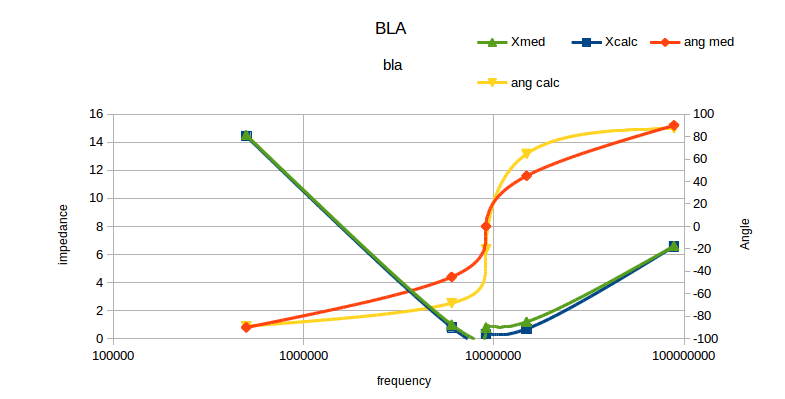
\includegraphics[width=8cm]{Imagenes/comparacionCapacitorFinal.png}
			\caption{comparación entre modelo capcitor y mediciones vs 
			frecuencia.}
			\label{img:001} 
		\end{figure}

		\indent Se puede observar que el modelo se condice con lo medido.

\newpage
\section{Conclusiones}
	\indent A partir de las experiencias realizadas, lo primero que debe 
	advertirse es el comportamiento no ideal de aquellos componentes (
	resistencias, capacitores, inductancias, etc) respecto de la frecuencia de 
	operaci\'on. A modo de ejemplo, en este trabajo se ha visto que en altas 
	frecuencias las inductancias par\'asitas de los capacitores tienen un efecto
	dominante y el componente se comporta como un inductor. Un efecto similar 
	ocurre con las bobinas, cuyo comportamiento es el de un capacitor por encima
	de la frecuencia de resonancia. \\
	\indent El conocimiento del comportamiento de cada componente cuando var\'ia
	la frecuencia permite obtener modelos m\'as refinados del mismo y de esta 
	forma un entendimiento m\'as amplio de su operaci\'on. Evidentemente esto 
	est\'a relacionado con la tecnolog\'ia de cada componente, es decir, 
	dependiendo de c\'omo se fabrique, \'este se comportar\'a idealmente en un 
	rango de frecuencias m\'as o menos amplio. \\
	\indent A los fines de realizar un dise\~no electr\'onico, es importante 
	caracterizar a los componentes, para que su funcionamiento sea el previsto. 
	Para ello existe diferente instrumental disponible (Q-metro, puente de 
	impedancias, RLC, impedanc\'imetro, etc) dependiendo de qu\'e par\'ametro se
	desee conocer. Es importante destacar este \'ultimo punto ya que, c\'omo se 
	ha mostrado en este trabajo, no todos los instrumentos tiene el mismo grado 
	de exactitud al realizar determinada medici\'on. Con lo cu\'al es importante
	saber c\'uando usar cada instrumento. A modo de ejemplo tanto el RLC como el
	impedanc\'imetro pueden medir la resistencia serie de un capacitor, sin 
	embargo con el primer instrumento se obtiene con una incerteza del $0.05 \%$
	mientras que con el impedanc\'imetro \'esta es del orden del $100\%$. Por 
	otra parte el rango de frecuencias donde eval\'ua el RLC es menor al del 
	impedanc\'imetro. \\	
	\indent Se concluye que la realizaci\'on de este trabajo permiti\'o la 
	adquisici\'on de criterio para utilizar diferente instrumental seg\'un sea 
	requerido\\
\end{document}

